\documentclass[11pt]{article}
\usepackage[small]{titlesec}
\usepackage[top = 0.66in,textwidth = 6.5in, textheight=9.1in]{geometry}

\usepackage{amsmath}
\usepackage{graphicx}
\usepackage{latexsym}
\usepackage{color}
\usepackage{amssymb}
\usepackage{tabularx}
\usepackage{fancyhdr}
\usepackage{verbatim}
\usepackage{multirow}
\usepackage{framed}
\usepackage{natbib}
\usepackage{float, subfig}
\usepackage{enumitem}
\usepackage{mathtools}
\usepackage{mathrsfs}
\usepackage{amsfonts}
\usepackage{listings}
\usepackage{amsthm}
\usepackage{grffile}
\usepackage{sidecap}
\usepackage{pbox}
\usepackage{algorithm}
\usepackage{longtable}
\usepackage[noend]{algpseudocode}

\def\qed{\hfill{\(\vcenter{\hrule height1pt \hbox{\vrule width1pt height5pt
     \kern5pt \vrule width1pt} \hrule height1pt}\)} \medskip}

\newtheorem{theorem}{Theorem}
\newtheorem{lemma}[theorem]{Lemma}
\newtheorem{corollary}[theorem]{Corollary}
\newtheorem{proposition}[theorem]{Proposition}
\newtheorem{conjecture}[theorem]{Conjecture}
\newtheorem{remark}{Remark}
\newtheorem{example}{Example}
\newtheorem{definition}{Definition}
\renewcommand{\textfraction}{0.0}
\newcommand{\dst}{\displaystyle}
\newcommand{\minx}{\mbox{\( \dst \min_{x \in X} \)}}
\newcommand{\Efx}{\mbox{\( \dst E f (x, \xi) \)}}
\newcommand{\Efxhat}{\mbox{\( \dst E f (\hat{x}, \xi) \)}}
\newcommand{\hxx}{\mbox{\( \hat{x} \)}}
\newcommand{\bpi}{\bar{\pi}}
\newcommand{\xx}{\mbox{\( x \)}}
\newcommand{\txxi}{\mbox{\(\xi\)}}
\newcommand{\var}{\mbox{var}}
\newcommand{\cF}{{\cal F}}
\newcommand{\cG}{{\cal G}}
\newcommand{\cN}{{\cal N}}
\newcommand{\cO}{{\cal O}}
\newcommand{\txi}{{\xi}}
\newcommand{\PP}{\mbox{\(SP\)}}
\newcommand{\PPn}{\mbox{\(SP_n\)}}
\newcommand{\PPnx}{\mbox{\(SP_{n_x}\)}}
\newcommand{\noi}{\noindent}
\renewcommand{\ss}{\smallskip}
\newcommand{\ms}{\medskip}
\newcommand{\bs}{\bigskip}
\newcommand{\st}{\mbox{s.t.}}
\newcommand{\wpo}{\mbox{wp1}}
\newcommand{\iid}{\mbox{i.i.d.\ }}
\newcommand{\vsmo}{\vspace*{-0.1in}}
\newcommand{\vsmt}{\vspace*{-0.2in}}
\newcommand{\vso}{\vspace*{0.1in}}
\newcommand{\vst}{\vspace*{0.2in}}
\newcommand{\mc}{\multicolumn}
\newcommand{\cP}{{\cal P}}
\newcommand{\underv}{\mbox{$\underbar{$v$}$}}
\allowdisplaybreaks 

\renewcommand{\P}{{\mathbb P}}
\newcommand{\E}{{\mathbb E}}
\newcommand{\R}{{\mathbb R}}
\renewcommand{\Re}{{\mathbb R}}
\newcommand{\mbf}{\mathbf}

\bibliographystyle{plain}

\begin{document}
%0.27
\baselineskip0.25in

\begin{center}
\begin{large}
\begin{bf}

Optimal Crashing of a PERT Network with Disruptions \ms

\today \ms
\end{bf}
\end{large}
\end{center}

\section{Introduction} \label{sec:introduction}
	The management of complex projects through optimization has a rich history in operations research, beginning with the program evaluation and review technique (PERT) \cite{malcolm1959application} and the critical path method (CPM) of \cite{kelley1961criticalpath}; see S{\"o}derlund \cite{soderlund2004building} for an overview and see \cite{Elmaghraby77}. To formulate a mathematical model, a project is viewed as a collection of activities, each of which has some duration and may consume some resources. There are precedence relationships between activities due to logical or technological considerations. The objective is to complete all activities in minimum time. We represent such a project using an acyclic activity network, where the length of each link shows the duration of an activity, and an edge's predecessors capture the precedence relationships. An activity cannot start until all its predecessors are completed. Multiple activities can be processed at the same time without a upper limit, as long as the precedence requirement is satisfied. More details about the activity network are discussed in \cite{Elmaghraby77}.\\
	\newline 
	In the planning stage of a project, decisions are made to crash a certain set of activities in order to minimize the project's timespan. Here crashing an activity means shortening its duration. In this paper, a discrete set of crashing options are available, each with fraction specifying the resulting reduction in the activity's duration. An activity can be crashed at most once and with a single option. Each option incurs a certain cost, and the total cost of crashing cannot exceed the budget. Optimization of such static crashing problems is introduced in \cite{fulkerson1961network, kelley1961criticalpath}. Under a finite set of crashing options, the problem can be modeled as a mixed integer program. The static model can be extended to incorporate uncertainty of activity durations. Monte Carlo simulation methods are used to estimate the expected project span given distributions of activity lengths, since it is is difficult to express analytically the expected project span \cite{burt1971conditional,van1963letter}. Heuristics and simulation-based algorithms have been developed to solve the stochastic project crashing problem \cite{aghaie2009ant,bowman1994stochastic,ke2014genetic,kim2007heuristic}. Another approach to handle the uncertainty is robust optimization, in which the objective is to minimize the worst case project span within a specified uncertainty set. While affinely adaptive recourse decisions are computationally tractable as linear, or second-order cone, programs, this restriction may lead to suboptimal solutions \cite{chen2008linear,cohen2007stochastic}. However, once recourse decisions can take general form, the robust model is only tractable with hypercube uncertainty sets, which is a trivial case because the worst-case scenario in the uncertainty set is always the point where every activity takes its upper bound \cite{wiesemann2012robust}. Ahipasaoglu et al. \cite{ahipasaoglu2016distributionally} propose a distributionally robust optimization scheme applied to a PERT network, which reformulates the problem as a semidefinite program or a copositive program, depending on the description of uncertainty.\\
	\newline
	The uncertainty in our paper lies in the timing and the magnitude of the stochastic disruption, which is modeled differently from randomness in a two-stage stochastic program or from the uncertainty set in robust optimization. A stochastic disruption is an event that may occur any time in the time horizon and change the system parameters significantly. A few authors apply this idea when the disruption can only occur in a set of specified time periods. Yu and Qi \cite{yu2004disruptionmgt} introduce scenario-based optimization models for airline scheduling. Morton et al. \cite{morton2009sealift} introduce a sealift scheduling problem under a finite number of stochastic disruptions within a stochastic programming structure. This structure ``falls between standard two-stage and multi-stage stochastic programs for a multi-period problem" and reduces the size of the problem to a quadratic growth in the number of time periods. Our setting inherits the philosophy of \cite{morton2009sealift} but enhances the model by allowing a continuous disruption time instead of a prespecified set of fixed time periods. \\
	\newline
	We first formally describe the crashing optimization problem under stochastic disruptions. Given a limited number of disruption scenarios, the problem can be formulated as a stochastic mixed integer program and we present the extensive formulation in Section~\ref{sec:formulation}. If we assume a continuous distribution for the disruption time and magnitude, a sample average approximation (SAA) can be used to create a finite set of scenarios and approximate the original problem by a finite-sized optimization problem. We present some important properties of this problem using a serial activity network as a special case in Section~\ref{sec:examples}. 
	\begin{comment}
	We prove some important consistency and convergence properties of the SAA problem using independent and identically distributed samples and stratified samples in Section~\ref{sec:consistency}.\\
	\newline
	The large scale and the discrete non-convex nature of the SAA problem's extended formulation means it may not be solved efficiently to desirable tolerance level. In Section~\ref{sec:decomposition}, a branch-and-cut method based on Benders decomposition is developed to solve the crashing optimization problem with a disruption. We show such a decomposition method solves the integer program to the exactness within finite number of iterations.\\
	\newline
	The experiment results are presented in Section~\ref{sec:results}, including the comparison between the quality of our solution and the solution obtained by solving a  crashing optimization problem with a deterministic disruption, and the computational performance of the decomposition method in Section~\ref{sec:decomposition}, compared to that of solving the extensive formulation. We conclude our paper with remarks on potential extensions of this model in Section~\ref{sec:conclusions}.
	\end{comment}
	
\section{Problem Formulation} \label{sec:formulation}
	The deterministic project crashing optimization problem has been known since the 1960s \cite{fulkerson1961network, kelley1961criticalpath}. Suppose the activity network is represented by a directed graph \(\mathcal{G} = (I,\mathcal{A})\), where the set of activities is denoted by \(I\) and their precedence relationship is characterized by \(\mathcal{A}\). The arc \((i,j) \in \mathcal{A}\) indicates that activity \(i\) has to be finished before the start of activity \(j\). We create a dummy activity \(N\) to represent the end of entire project, which should succeed every activity \(i \in I\). \\
	\newline
	For each activity \(i \in I\), the nominal length \(D_i\) is given. We can apply a finite set of crashing options, \(j \in J_i\), and one unit application of each option incurs a cost of \(b_{ij}\), while it decreases the length of activity \(i\) by \(D_ie_{ij}\). The total cost of crashing options cannot exceed a given budget, \(B\). We assume each activity can be crashed at most with one unit and the problem can be formulated as follows:
	\begin{subequations} \label{prob2:static}
		\begin{align}
		\min \quad & t_N &\\
		\text{s.t.} \quad &  t_k - t_i \geq D_{i}(1 - \sum_{j \in J_i} x_{ij} e_{ij}) \qquad \qquad \forall \,i \in I, (i,k) \in \mathcal{A} \label{cons:dSep}\\
		& \sum_{i \in I} \sum_{j \in J_i} b_{ij}x_{ij} \leq B  \label{cons:dBudget}\\
		& \sum_{j \in J_i} x_{ij} \leq 1  \qquad \qquad \forall \,i \in I \label{cons:dSingleBudget}\\
		& t_i \geq 0  \qquad \qquad \forall \,i \in I\\
		& 0 \leq x_{ij} \leq 1  \qquad \qquad \forall \,i \in I, j \in J_i.
		\end{align}
	\end{subequations}
	In this formulation, \(t_i\) represents the starting time of activity \(i \in I\). We aim to minimize the project span, which is the starting time of the dummy activity, \(t_N\). Constraint~\eqref{cons:dSep} guarantees the precedence relationship: if activity \(i\) precedes activity \(k\), activity \(k\) cannot start until activity \(i\) is finished, since the finishing time of activity \(i\) is \(t_i + D_i (1- \sum_{j \in J_i} x_{ij}e_{ij})\). Constraint~\eqref{cons:dBudget} is the budget constraint and constraint~\eqref{cons:dSingleBudget} ensures that no more than one unit of crashing option can be applied to an activity. \\
	\newline
	In our problem, we assume at most one stochastic disruption can occur in the project span, while the time of such disruption is a random variable. We also assume for each activity \(i \in I\), the crashing decision decision for that activity needs to be made prior to the start of that activity, and cannot be changed after that. We assume that the disruption does not affect the activities that have already started but changes the length of activities starting after it according to some given distributions. We assume there is a discrete finite set of scenarios indexed by \(\Omega\). It is usually hard to compute the recourse function directly when some of its parameters are distributed according to continuous distributions, and SAA is proposed to approximate the problem by a large-scale deterministic optimization problem with a finite scenario set \cite{kim2015guide,shapiro2009lectures}. \\
	\newline
	Since there is at most one disruption, we can model the problem as a two-stage stochastic mixed integer program. Notice that the definition of the first stage is different from the traditional stochastic program setting. Here the first stage contains decisions through completion of the project if no disruption occurs and the second stage characterize the decisions for each realization of the disruption. This means that the first stage decision variables are carried out until the disruption, if it ever occurs, and after the disruption, depending on the scenario realized, the scenario-specific recourse decisions are executed.\\
	\newline
	The notation for the model is displayed as follows:
	\begin{longtable}[H]{ l l l l }
		\multicolumn{4}{l}{Indices and index sets} \\
		\\
		\(I\) & \(\qquad\) & the set of activities;&\\
		\(J_i\) & \(\qquad\) & the set of crashing options for activity \(i\), \(i \in I\);&\\
		\(\Omega\) & \(\qquad\) & the index set of possible realizations of disruption;&\\
		\(\mathcal{A}\) &\(\qquad\) & set of arcs which represents the precedence relationship;&\\
		\\
		\multicolumn{4}{l}{Parameters} \\
		\\
		\(D_{i}\)& \(\qquad\) & original duration of activity \(i\), \(i \in I\);&\\
		\(e_{ij}\) & \(\qquad\) & effectiveness of crashing option \(j\), \(i \in I, j \in J_i\);&\\
		\(B\) & \(\qquad\) & total budget;&\\
		\(b_{ij}\) & \(\qquad\) & cost of crashing option \(j\), \(i \in I, j \in J_i\);&\\
		\(H^\omega\) &\(\qquad\) & disruption time in scenario \(\omega\), \(\omega \in \Omega\);&\\
		\(d_{i}^\omega\) & \(\qquad\)&the change of duration of activity \(i\) in realization \(\omega\), &\\
		& \(\qquad\) & if the activity is started after the disruption, \(i \in I, \omega \in \Omega\);& \\
		\(p^\omega\) & \(\qquad\) & the probability of scenario \(\omega\), \(\omega \in \Omega\);& \\
		\(p^0\) & \(\qquad\) & the probability of no disruption;& \\
		\\
		\multicolumn{4}{l}{Decision Variables}\\
		\\
		\(t_{i}\) & \(\qquad\) & nominal starting time of activity \(i\), \(i \in I\);&\\
		\(x_{ij}\) & \(\qquad\) & fraction activity \(i\) is crashed by option \(j\) in the nominal plan, \(i \in I, j \in J_i\); &\\
		\(t_{i}^\omega\) & \(\qquad\) & starting time of activity \(i\) under scenario \(\omega\), \(i \in I, \omega \in \Omega\);&\\
		\(x_{ij}^\omega\) & \(\qquad\) & fraction activity \(i\) is crashed by option \(j\) under scenario \(\omega\), \(i \in I, j \in J_i, \omega \in \Omega \); &\\
		\(G_i^\omega\) & \(\qquad\) & indicator whether activity \(i\) starts after disruption in realization \(\omega\), \(i \in I, \omega \in \Omega\);&\\
		\(S_{ij}^\omega\) & \(\qquad\) & binary term to linearize the bilinear term \(G_i^\omega x_{ij}^\omega\), \(i \in I, j \in J_{i}, \omega \in \Omega\).&\\
	\end{longtable}
	\noi The extensive formulation of the two-stage stochastic program is shown as formulation~(\ref{prob2:extensive}):
	\begin{subequations} \label{prob2:extensive}
		\begin{align}
		\min \quad & \sum_{\omega \in \Omega} p^\omega t_N^\omega + p^0 t_N \\
		\text{s.t.} \quad & t_N^\omega \geq t_i^\omega \qquad \qquad \forall \,i \in I, \omega \in \Omega \\
		& t_N \geq t_i \qquad \qquad \label{cons:tN}\\
		& t_i^\omega \geq 0 \qquad \qquad \forall \,i \in I, \omega \in \Omega\\
		& t_i \geq 0 \qquad \qquad \forall \,i \in I\\
		& H^\omega - (1 - G_i^\omega) M \leq t_i \qquad \qquad \forall \,i \in I, \omega \in \Omega \label{cons:F}\\
		& H^\omega + G_i^\omega M \geq t_i \qquad \qquad \forall \,i \in I, \omega \in \Omega \label{cons:G}\\
		& t_i^\omega + G_i^\omega M \geq t_i \qquad \qquad \forall \,i \in I, \omega \in \Omega \label{cons:tf1}\\
		& t_i^\omega - G_i^\omega M \leq t_i \qquad \qquad \forall \,i \in I, \omega \in \Omega \label{cons:tf2}\\
		& x_{ij}^\omega + G_i^\omega \geq x_{ij} \qquad \qquad \forall \,i \in I, j \in J_i, \omega \in \Omega \label{cons:xf1}\\
		& x_{ij}^\omega - G_i^\omega \leq x_{ij} \qquad \qquad \forall \,i \in I, j \in J_i, \omega \in \Omega \label{cons:xf2}\\
		& t_k^\omega - t_i^\omega \geq D_i + d_i^\omega G_i^\omega -\sum_{j \in J_i} D_i e_{ij} x_{ij}^\omega - \sum_{j \in J_i} d_i^\omega e_{ij} S_{ij}^\omega \qquad \qquad \forall \,i \in I, j \in J_i, \omega \in \Omega \label{cons:duration}\\
		& \sum_{j \in J_i} x_{ij}^\omega \leq 1 \qquad \qquad \forall \,i \in I, \omega \in \Omega \label{cons:crashLim}\\
		& \sum_{i \in I}\sum_{j \in J_i} b_jx_{ij}^\omega \leq B \qquad \qquad \forall \,\omega \in \Omega \label{cons:budget}\\
		& S_{ij}^\omega \leq G_i^\omega \qquad \qquad \forall \,i \in I, j \in J_i, \omega \in \Omega \label{cons:linearize1}\\
		& S_{ij}^\omega \leq x_{ij}^\omega \qquad \qquad \forall \,i \in I, j \in J_i, \omega \in \Omega \label{cons:linearize2}\\
		& S_{ij}^\omega \geq G_i^\omega + x_{ij}^\omega - 1 \qquad \qquad \forall \,i \in I, j \in J_i, \omega \in \Omega \label{cons:linearize3}\\
		& t_i^\omega \geq H^\omega G_i^\omega \qquad \qquad \forall\, i \in I, \omega \in \Omega \\
		& 0 \leq x_{ij} \leq 1 \qquad \qquad \forall \,i \in I, j \in J_i\\ 
		& 0 \leq x_{ij}^\omega \leq 1 \qquad \qquad \forall \,i \in I, j \in J_i, \omega \in \Omega\\
		& 0 \leq S_{ij}^\omega \leq 1 \qquad \qquad \forall \,i \in I, j \in J_i, \omega \in \Omega\\
		& G_i^\omega \in \{0,1\}. \qquad \qquad \forall \,i \in I, \omega \in \Omega.
		\end{align}
	\end{subequations}
	In model~\eqref{prob2:extensive}, we are minimizing the expected project span by taking the sum of each scenario's project span weighted by the scenario probability. Variables \(G^\omega_i\) are used to identify whether activity \(i\) starts before or after the disruption time (in constraint \eqref{cons:F}-\eqref{cons:G}) and \(M\) is a large number to enforce the logic relationships. This is important in our problem setting because the duration of each activity depends on its temporal relationship to the disruption time, which is reflected in constraint (\ref{cons:duration}). For this duration constraint, the original expression of the duration of activity \(i\) is \((D_i + d_i^\omega G_i^\omega)(1 - \sum_{j \in J_i} e_{ij}x_{ij}^\omega)\). This contains a bilinear term \(G_i^\omega x_{ij}^\omega\), which is linearized by introducing a binary variable \(S_{ij}^\omega\) and bounding it by constraints \eqref{cons:linearize1}-\eqref{cons:linearize3}.\\
	\newline
	We use a set of non-anticipativity constraints \eqref{cons:tf1}-\eqref{cons:xf2}, different from ones used in a traditional stochastic programming because the first stage decision variables here spans the entire time horizon. These logic constraints ensure that the decisions made before the disruption time in each scenario are the same as the nominal decisions before the same time point.
	
\section{Special Cases} \label{sec:examples}
	In this section we show a serial example to illustrate the nature of the project crashing problem under stochastic disruption. From this serial network example we show that it might be optimal to delay the start of some activities, and thus justify the formulation in model~\eqref{prob2:extensive}. \\
	\newline
	Suppose we have a project with three activities in a serial network form. Activity 1 must finish before the start of activity 2 and the activity 2 must finish before the start of activity 3. The structure of the project is displayed as follows. We add a dummy activity ``N" to represent the end of the project. The total crashing budget is \(1\) and the allowed amount of crashing a single activity is between \(0\) and \(1\). 
	\begin{figure}[H]
		\centering
		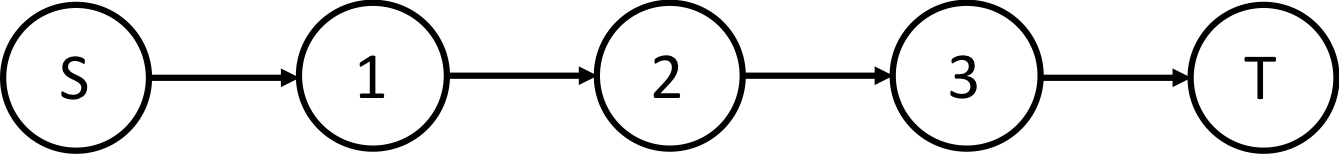
\includegraphics[width=0.8\textwidth]{serial3}
		\caption{Example of a 3-activity project}
		\label{fig:serial3}
	\end{figure}
	\noi So, \(I=\{1,2,3,N\}\), and \(D_1=9\), \(D_2=10\), and \(D_3=7\). The probability of the disruption not occurring is \(p^0=\frac{1}{2}\), and if a disruption occurs, it will occur at the time \(H^2 = 9.1\). The set of scenario \(\Omega = \{1\}\), where scenario 1 represents the disruption scenario. Suppose the disruption changes \(D_2=10\) to \(3\), a.k.a. \(d_2^1 = -7\), and not affect activity 3. We can see it is optimal to delay the start of activity 2 to \(t_2 = 9.1\), spend the entire budget to crash activity 3 if the disruption occurs, and spend the entire budget to crash activity 2 if the disruption does not occur. The expected total project span is 18.35. If we force the condition that the starting time of activities cannot be delayed, we cannot observe whether the disruption happens or not prior to the start of activity 2. There is only one possible situation where three activities have the duration as 9, 10 and 7. All resources should be allocated to activity 2 and the total project span is 21, which is larger than the expected total project span if it is allowed to delay the starting time of some activities. In this example, a disruption may reduce the duration of some activities and delaying by a small amount allows us to realize that reduction in time.\\
	\newline
	Even if the disruption can only lengthen an activity's duration, it is still beneficial to delay the start of some activities under some circumstances. This means a small delay of some activity may gain the information regarding the disruption, which can decrease the project span. To see this, we again consider the serial network of Figure~\ref{fig:serial3}. We assume the nominal durations, and the stochastic disruption, are identical to those above. If the disruption occurs, the durations of activities change by \(d_2^1=0.1\) and \(d_3^1 = 6\). For this example, if no delay is allowed, the optimal decision is to have \(x_2 = 1\) and the optimal objective value is 24. If we delay the starting time of the activity 2 to \(t_2 = 9.1\) so that the disruption can be observed before we commit resources to activity 2, the optimal expected total project span is 23.4. \\
	\newline
	Because it is possible for an optimal crashing plan to contain a delay for some activities, we have to set up decision variables \(t_i,\ \forall i \in I\), as the starting time of each activity, rather than assume that each activity starts as soon as all of its predecessors are finished.  We summarize the reasons of such delay include:
		\begin{enumerate}
			\item Some activities might have a shorter length after disruption. It is beneficial to wait a short period of time to capture this advantage.
			\item Even if all possible disruption magnitudes are adverse, which means they lengthen all activities, it is beneficial to delay an activity so that the crashing resource could be optimally applied according to the realization of disruption.
		\end{enumerate}
	\begin{comment}
	\textcolor{blue}{ The materials above are the most important idea I want to convey in this section. Here are some additional results we have discussed but I haven't compiled to \LaTeX \ yet. Time allowing, I can add some stuff in maybe tonight or this coming week.
		\begin{itemize}
			\item Concavity of \(\mathbb{E}_d \left[ f(x,H,d) | H \right]\) in \(d\).
			\item The analytical form of the recourse function when all \(d\) are \([0,1]\)-uniformly distributed, all \(D\) are equal, and the crashing option can only be integer.
			\item The recourse function is a decreasing function in terms of remaining budget, given the same remaining task set.
			\item Not optimal to delay the start of activity \(i\) unless there is no investment before \(i\), given a fixed \(H\).
			\item Only optimal to delay to a possible disruption time.
		\end{itemize}
	}
	\subsection{Parallel Networks}
		\begin{itemize}
			\item Not optimal to delay when \(d_i \geq 0\) if each branch only contains a single activity.
			\item If each branch is a serial path, it is possibly beneficial to delay the start of some activities.
		\end{itemize}
	\subsection{Y Networks}
\section{Properties of the Sample Average Approximation Problem} \label{sec:consistency}
	\subsection{Cheat?}
	\subsection{Consistency and Convergence Results}
	\subsection{IID vs. Stratified Sampling}
\section{Decomposition Method} \label{sec:decomposition}
	Problem~\eqref{prob2:extensive} is a two-stage stochastic mixed integer program with binary variables in the second stage. 
	
\section{Experiment Results} \label{sec:results}
	\subsection{Deterministic Counterparts}
		List the test results of INFORMS presentation. State the fact that the fully stochastic makes great improvement over its deterministic counterparts.
		
%\section{Stochastic Mixed Integer Program Extension}
\section{Conclusions} \label{sec:conclusions}
\end{comment}

\bibliographystyle{plain}
\bibliography{PERT_Bib}

\end{document}